\documentclass[tikz,border=10pt]{standalone}
\usepackage{tikz}
\usetikzlibrary{calc,angles,quotes}

\begin{document}

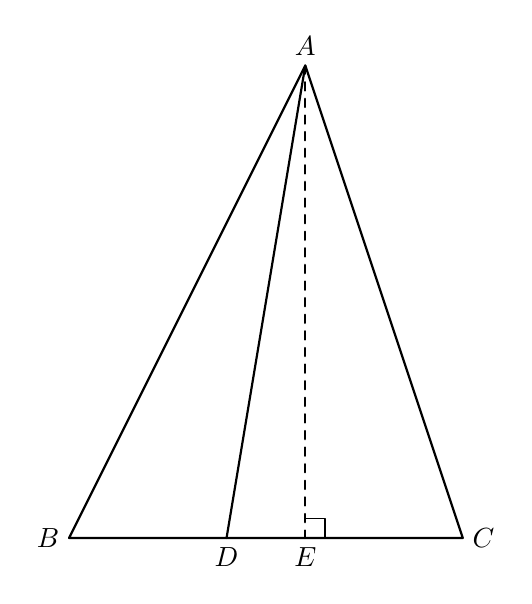
\begin{tikzpicture}[line cap=round, line join=round, >=stealth, x=1cm, y=1cm]
    % ---------------------------------------------------------
    % 1. 定义坐标点 (由图像形态推算比例)
    % ---------------------------------------------------------
    \coordinate (B) at (0,0);
    \coordinate (C) at (5,0);
    \coordinate (A) at (3,6);     % 顶点 A 略微偏右
    \coordinate (E) at (3,0);     % 垂足 E，垂直于 BC
    \coordinate (D) at (2,0);     % D 点位于 B 和 E 之间

    % ---------------------------------------------------------
    % 2. 绘制图形边界
    % ---------------------------------------------------------
    % 绘制三角形 ABC
    \draw[thick] (A) -- (B) -- (C) -- cycle;
    
    % 绘制内部实线 AD
    \draw[thick] (A) -- (D);
    
    % 绘制辅助高线 AE (虚线)
    \draw[dashed, thick] (A) -- (E);

    % ---------------------------------------------------------
    % 3. 绘制垂直符号
    % ---------------------------------------------------------
    % 绘制 E 点处的直角标志
    \draw (E) ++(0, 0.25) -- ++(0.25, 0) -- ++(0, -0.25);

    % ---------------------------------------------------------
    % 4. 标注字母节点
    % ---------------------------------------------------------
    % 调整节点位置以符合图片中的视觉效果
    \node [above] at (A) {$A$};
    \node [left]  at (B) {$B$};
    \node [below] at (D) {$D$};
    \node [below] at (E) {$E$};
    \node [right] at (C) {$C$};

\end{tikzpicture}

\end{document}